% Chapter Template

\chapter{Quantitative Analysis} \label{sec:chapter3} % Main chapter title
%this should end up being roughly 15-20 pages


\label{Chapter3} % Change X to a consecutive number; for referencing this chapter elsewhere, use \ref{ChapterX}

%----------------------------------------------------------------------------------------
%	SECTION 1
%----------------------------------------------------------------------------------------


\section{Data \& Methods}
The primary objective of this work is to predict if a riot or protest will occur in a specific urban area, based solely on data from satellite imagery.  In order to accomplish this objective, we leverage convolutional neural networks in combination with two data sources, ACLED \citep{ACLED} and Planet \citep{planet}. We use these data to generate two different sets of information: the first set is satellite imagery of locations where riots occurred, and the second is a set of images of proximate areas (within the same city) that did not experience a riot event.  Our deep learning model then seeks to disambiguate between these two cases, based on satellite imagery alone. This section provides details of our data processing and analytic approach.

\subsection{Data} \label{sec:data_paper1}
\subsubsection{Selecting Riot Locations}
Determining the locations where riots and protests have occurred is the first step in developing a data set for this work.  To identify these locations, we leverage the Armed Conflict Location Event Data Project (ACLED), an open source database which contains information on a wide range of conflict types from across the globe \citep{ACLED}.  ACLED contains more than 1.5 million events from 1997 to 2023, which are aggregated, categorized, and curated to create a data source that can specify time and location for conflict.  We filter this database according to a number of criteria:
\begin{enumerate}[topsep=0pt,itemsep=-1ex,partopsep=0ex,parsep=0.5ex]
\item \textbf{Type of event. } We focus our analysis on protests and riots, which primarily represent urban unrest.
\item \textbf{Date. } We only leverage protest or riot events with a known date of occurrence.
\item \textbf{Geography. } Only events with a known neighborhood-level geographic footprint are selected.\footnote{For example, some riots are known to have occurred in Beriut, while others occurred within neighborhoods in Beriut. There are 12 neighborhoods listed within some of the ALCED entries for Beriut (Ras Beirut, Port, Mazraa, Achrafieh, Mousseitbeh, Saifi, Minet El Hosn, Rmeil, Bachoura, Medawar, Ain Mreisseh, and Zokak El Blat).  These neighborhood specific entries have neighborhood specific latitudes and longitudes, and we use these neighborhood specific events to construct our data set.}
\end{enumerate}

After filtering events, we are left with a resultant database of 53,307 events. In order to prevent over representation of any single unique location in the database, a maximum of 500 events were randomly selected from each neighborhood (i.e., "Seoul - Jongno"). After this stage, a total of 37,728 events across 1,089 unique locations were leveraged to construct our dataset of the location of conflict events.






\subsubsection{Satellite Data}
Once we have identified the location of riot events, we retrieve relevant \textit{Planetscope} satellite imagery both (a) 24-48 hours prior to each event, and (b) in similar, nearby geographic locations that did not experience unrest.  Planetscope - an integrated collection of images from the Dove, Dove-R and SuperDove satellites - provides four-band (RGB and NIR), approximately three to four meter spatial resolution satellite imagery with a daily temporal resolution (\cite{planetScope}; see table \ref{tab:planetscope}). For both cases of imagery (with and without riot), we consider images that contain less than 50\% cloud cover.  An example of the imagery available can be seen in figure \ref{fig:athens_baseimage}.  


\begin{table}
    \centering
    \begin{tabular}{|l|c|c|c|}
    \hline
            & \textbf{Dove Classic} & \textbf{Dove-R} & \textbf{SuperDove}\\
         Band  & Wavelength (nm) & Wavelength (nm) & Wavelength (nm) \\
         \hline
         Red   & 590 - 670       & 650 - 682       & 650 - 680\\
         Green & 500 - 590       & 547 - 585       & 547 - 583\\
         Blue  & 455 - 515       & 464 - 517       & 465 - 515\\
         \hline
    \end{tabular}
    \caption{Technical wavelength specifications for RGB bands of Planetscope sensors \citep{planetScope}.  }
    \label{tab:planetscope}
\end{table}

\begin{figure}
    \centering
    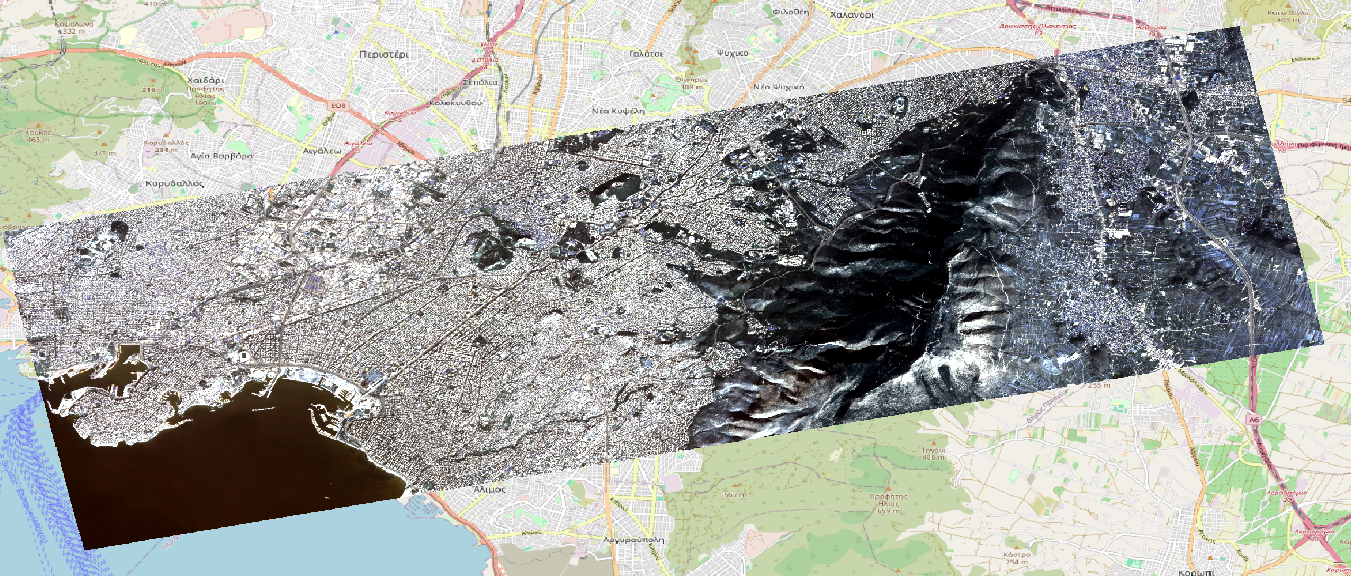
\includegraphics[width=1\linewidth]{athens_greece_satimage.png}
    \caption{Satellite Image of Athens Greece, taken 31 January 2018. Imagery \textcopyright Planet Labs PBC 2023. All rights reserved.}
    \label{fig:athens_baseimage}
\end{figure}


\begin{table}[htbp]
    \centering
    \caption{PlanetScope Constellation \citep{planetScope} }
    \begin{tabular}{|l|l|l|}
        \hline
        \textbf{Instrument} & \textbf{Image area} & \textbf{Availability} \\
        \hline
        Dove Classic & 25 x 11.5 sq km & July 2014 - April 2022 \\
        Dove-R & 25 x 23 sq km & March 2019 - April 2022 \\
        SuperDove & 32.5 x 19.6 sq km & March 2020 - present \\

        \hline  
    \end{tabular}
    \label{tab:doves}
\end{table}


For each of the 37,728 instances of riots in our filtered ACLED dataset, we first retrieve a full scene of imagery from 24-48 hours prior to the event.  These scenes are guaranteed to encompass the latitude and longitude representing the centroid of the neighborhood at which a conflict occurred; in cases where multiple images were available for a given event we chose the one closest in time to the event (with a minimum of 24 hours prior to the event).  Ultimately, this process resulted in 19,902 satellite scenes being downloaded, with an average spatial dimension that can vary depending on the generation of satellite (see table \ref{tab:doves}) and geographic latitude of collection. Because riots may occur at the same location, but at multiple points in time, some locations (i.e., a seat of government, culturally significant locations, etc) may appear in the database multiple times; the most common of these occurrences are summarized in table \ref{tab:occurrence}.


\begin{table}[htbp]
    \centering
    
    \begin{tabular}{|l|l|l|l|l|}
        \hline
        \textbf{Country} & \textbf{Neighborhood} & \textbf{Count} & \textbf{Earliest Date} & \textbf{Latest Date} \\
        \hline
        Pakistan & Karachi - Saddar &  278 & 7 October 2017 & 30 September 2022 \\
        Iran & Tehran - District 6 &  270 & 9 October 2017 & 26 September 2022 \\
        Iran & Tehran - District 12 & 268 & 9 October 2017 & 28 September 2022 \\
        Lebanon & Beirut - Port & 252 & 7 October 2017 & 26 September 2022 \\
        Greece & Athens - Central Athens & 247 & 18 January 2018 & 28 September 2022 \\
        South Korea & Seoul - Jongno &  240 & 18 January 2018 & 21 September 2022 \\
        South Korea & Seoul - Jung & 226 & 18 January 2018 & 26 September 2022 \\
        Italy & Rome - City Center &  222 & 7 January 2018 & 23 September 2022 \\
        India & Delhi - New Delhi &  220 & 2 October 2017 & 4 September 2022\\
        South Korea & Seoul - Seocho & 220 & 8 January 2018 & 28 September 2022 \\
        \hline
    \end{tabular}
    \caption{Neighborhood locations which occur most frequently.  `Earliest' and `Latest' date refer to the earliest and latest date of a protest event for each neighborhood.  For example, in the neighborhood of Seocho in Seoul, 220 independent protest or riot events occurred from January 8th, 2018 to September 28th, 2022.  In our analysis, this would be represented by 220 individual satellite tiles, each taken between 24 and 48 hours before the actual event.}
    \label{tab:occurrence}
\end{table}



From the satellite scene retrieved for each conflict event, we extract two types of data.  First, we extract a one kilometer by one kilometer box centered on the conflict event neighborhood.  This box is saved and identified as the location of the unrest in our database.

Second, we extract a number of cases to serve as null events - i.e., locations from the same urban area, but where no unrest occurred.  To generate these null cases, we follow a multiple step process in which we:

\begin{enumerate}[topsep=0pt,itemsep=-1ex,partopsep=0ex,parsep=0.5ex]
\item \textbf{Identify urban areas. } We only consider areas in the scene that have a population density over 300 inhabitants per kilometer.
\item \textbf{Exclude areas that are within 10km of the conflict event. } We isolate the conflict event by removing the urban areas that are within ten kilometers of the centroid of the neighborhood in which conflict occurred.
\item \textbf{Sample. } With the remaining urban areas in the satellite scene, we generate a list of random centroids which are constrained to be a minimum of 2 kilometers apart, and select a maximum of 10 of these to generate 1km box `null' locations at which no protest or conflict occurred.  The 2 kilometer separation ensures that none of our null boxes overlap.
\end{enumerate}


In step one, we overlay information about the degree of urbanization \citep{ghs_smod_2023, urbanisation_manual_2021} onto each satellite scene to determine what portions are urban, and which parts are not.  This is accomplished by using the DEGURB dataset \citep{ghs_smod_2023}, which was developed by the European Commission's Joint Research Centre.  This data categorizes geographical areas into Urban Centre, Urban Clusters (including towns and suburbs), and Rural Grid Cells (including villages and dispersed rural) zones based on population density and contiguity of dense areas \citep{urbanisation_manual_2021}.  Its creation involves analyzing high-resolution satellite imagery and detailed population survey data, with the goal of providing an accurate representation of the urban landscape with one kilometer spatial resolution \citep{urbanisation_manual_2021}. The DEGURB dataset used in this work is representative of 2020 \citep{ghs_smod_2023}.  For our purposes we consider anything with a density over 300 inhabitants per square kilometer as urban \citep{urbanisation_manual_2021}.   The results of this approach are illustrated in figure \ref{fig:degurb}.  This binary representation of urban areas is then be applied to each satellite scene as a mask, allowing us to select null cases from proximate urban areas.

\begin{figure}
    \centering
    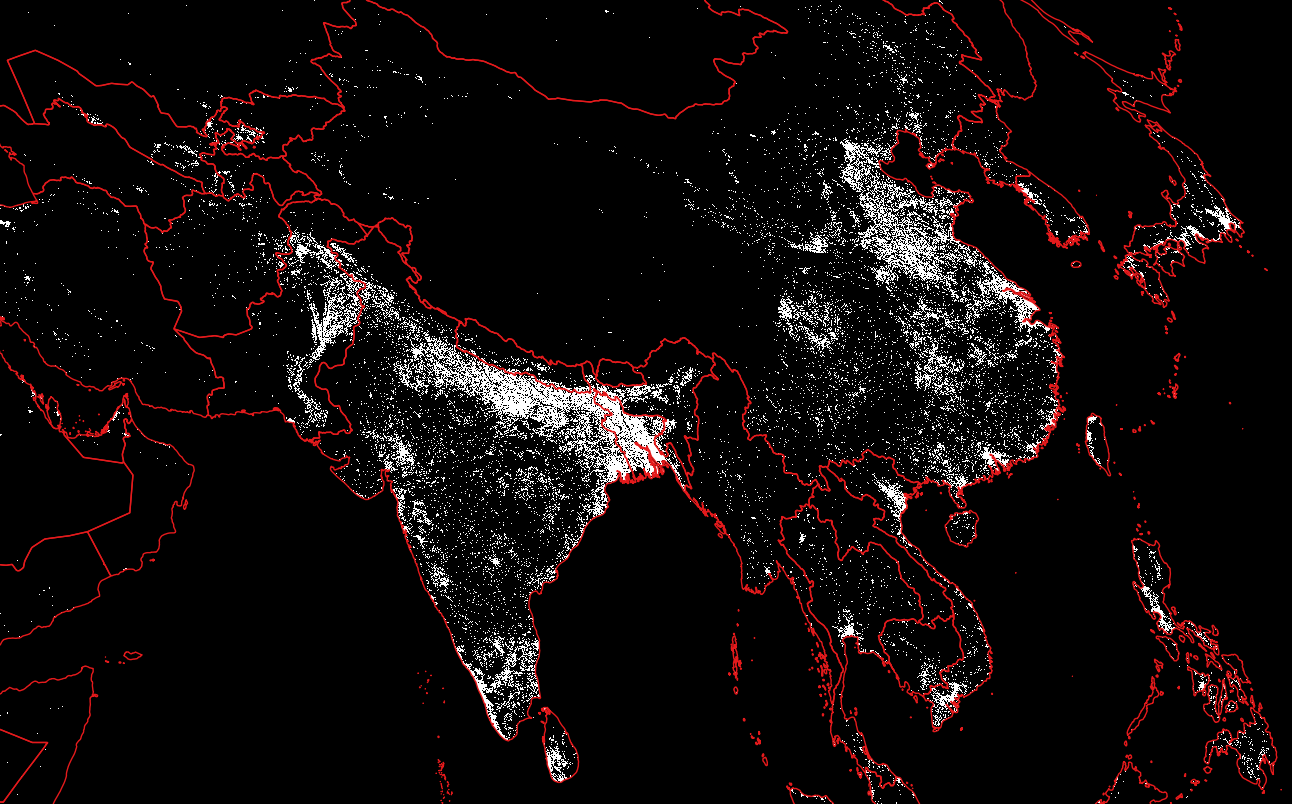
\includegraphics[width=0.9\linewidth]{degurb_B.png}
    \caption{A portion of the DEGURB data, highlighting areas of the world that are considered urban in our data set. DEGURB defines urban regions as those with a density more than 300 inhabitants per km \cite{urbanisation_manual_2021}.  Red lines represent country level boundaries \citep{runfola2020geoboundaries}.  }
    \label{fig:degurb}
\end{figure}


In step two, in order to ensure the areas selected for null cases are distinct from the areas of unrest, we exclude all urban areas up to 10 kilometers away from the centroid of the riot neighborhood from consideration, as illustrated in figure \ref{fig:athens_nullclips}.




Third, after excluding the ten kilometer region around each unrest event, from the remaining urban regions in the satellite scene we select random locations for null-riots.  We accomplish this by generating a list of random latitudes and longitudes that are within the available regions.  We ensure that each of these random locations are at least 2 kilometers away from any other locations on our random list.  We then take a maximum of ten of these locations, and construct a 1 kilometer box around each one.  We construct up to 10 null cases (that do not overlap) from the eligible urban regions from each scene (noting that less dense urban areas are occasionally represented by less than 10 null cases due to a lack of proximate urban areas). A visualization of the results from this process can be seen in figure \ref{fig:athens_nullclips}.

  

\begin{figure}
    \centering
    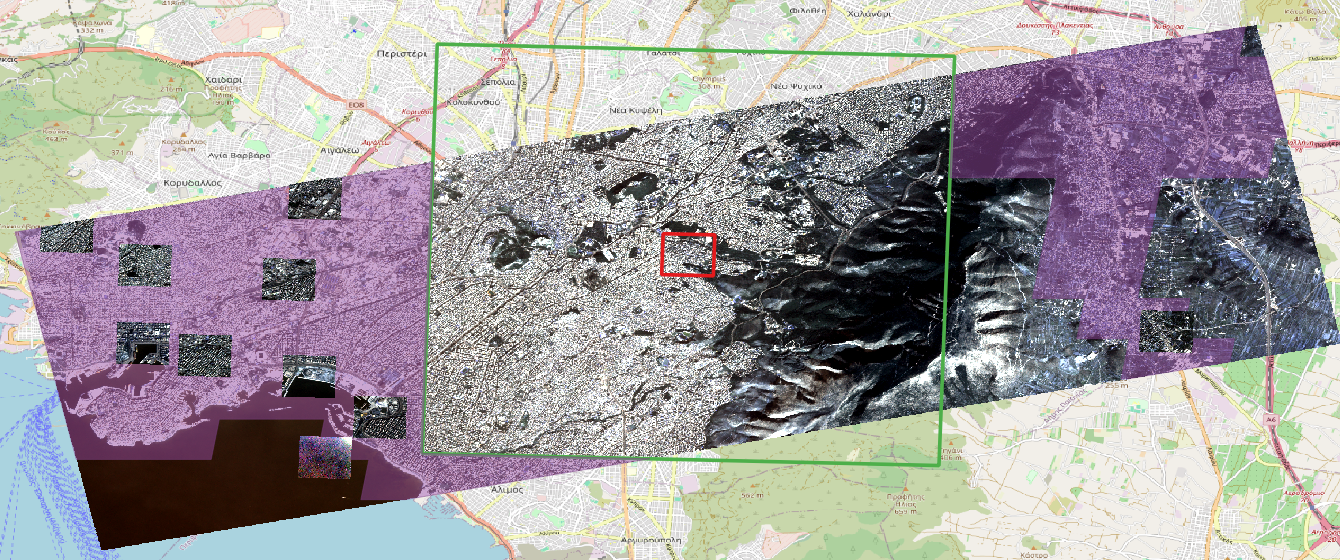
\includegraphics[width=0.9\linewidth]{athens_greece_nullclips.png}
    \caption{Satellite Image of Athens Greece, taken 31 January 2018.  The red box in the center of the image is a 1 kilometer box around the riot location.  The green box is a 10 kilometer exclusionary area around the riot location, from which we do not draw "null" case contrasts.  Areas which fall outside the green box, that are also urban, are eligible for selection (displayed  in purple).  From the potential null region, we sample random, non-overlapping 1 kilometer boxes to generate null location clips. Imagery \textcopyright Planet Labs PBC 2023. All rights reserved.}
    \label{fig:athens_nullclips}
\end{figure}



After this process is completed, for each conflict event we are left with a set of one ($\ 1 km^{2} $) kilometer box representative of where unrest occurred, and up to 10 ($\ 1 km^{2}$)  km boxes representative of urban areas proximate to the unrest event, but with no known activity.  Across our full dataset of 19,902 unrest locations, 18,634 (93.6\%) had 10 null cases available; the distribution of null cases across images can be seen in figure \ref{fig:null_hist}. Our final dataset included only locations that had the full complement of null clips, for a total of 18,631 cases of unrest, and 186,310 null cases. We then normalize all of these image clips based on a sample of the full satellite scenes \citep{goodman2021convolutional, runfola2022deep, lv2024mapping, brewer2023tracking}.  Tests of different permutations of this dataset (i.e., models with a 1:1 ratio of null and riot cases) can be found in section \ref{sec:limited_data_set}.



\subsection{Methods}\label{sec:methods_paper1}
Our overall modeling architecture is summarized in figure \ref{fig:flow_chart}. In order to estimate the likelihood of if an unrest event occurred or not at each location, we leverage a ResNet18 \citep{he2016deep} as our base model, replacing the fully connected layer with a series of dense layers with 128, 64, and 32 hidden nodes.  In order to improve the efficiency of our training, following other literature in the satellite imagery analysis space \citep{goodman2021convolutional, brewer2021predicting, runfola2022deep, lv2024mapping, brewer2023tracking}, pre-trained weights from ImageNet were used as our initial baseline. 

\begin{figure}
    \centering
    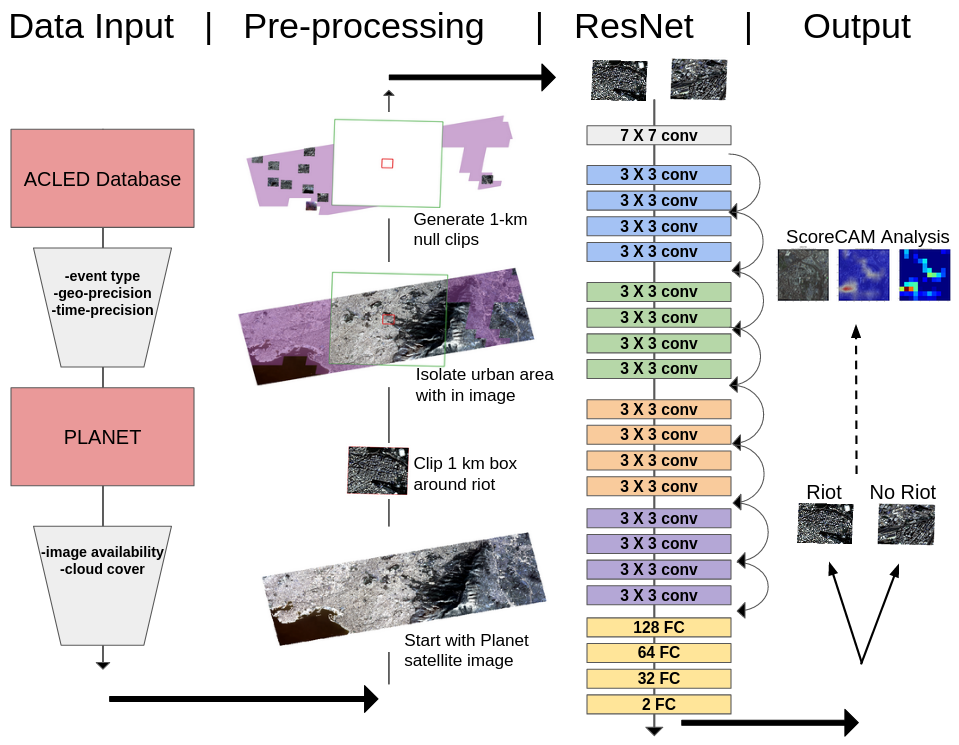
\includegraphics[width=0.75\linewidth]{flow_chart.png}
    \caption{A synopsis of our overall modeling architecture.  Stages include the collection of data, pre-processing, network training, categorization, and explainability analysis. Imagery \textcopyright Planet Labs PBC 2023. All rights reserved.}
    \label{fig:flow_chart}
\end{figure}

\subsubsection{Hyperparameter Search}
Prior to training on all 18,631 images, we first randomly selected a subset of 1,000 conflict events (1,000 unrest cases and 10,000 null cases) to implement a grid search across hyper-parameters \footnote{Training was performed using pyTorch on 8 RTX 6000 NVIDIA GPUs.  On average, models trained using the hyperparameter dataset took approximately 6.5 hours to complete 40 epochs; our full model across all images took 321 hours for 100 epochs.}. To account for class imbalance, we implement a weighted cross entropy loss \citep{ho2019real} with an ADAM optimizer \citep{kingma2014adam} for our training procedure.  

Our hyperparameter search encompassed trials of different learning rates, L2 regularization, dropout, freezing layers (results and parameters from a sample of the trials can be seen in the appendix in section \ref{large_table_of_results}).  Results from a selection of three of the best performing cases in the hyperparameter testing are shown in table \ref{tab:hyper_param_search}. On the basis of these results, we selected one model (denoted as Model C in table \ref{tab:hyper_param_search}) to test on the full dataset, which is described in table \ref{tab:fulldata_results_table}.
\par
We assess our model by interpreting the overall accuracy, precision and recall.  The precision is the ratio of true positives to the number of positive predictions our model made \citep{davis2006relationship}, which will measure our model's ability to correctly predict riots when it does makes a prediction.  The recall is the ratio of true positives to the number of riots in the data set, which measures our model's ability to identify how frequently riots are occurring \citep{davis2006relationship}.  

\begin{table}
\centering
\resizebox{\textwidth}{!}{%
\begin{tabular}{|l|p{1.5cm}|p{1cm}|p{2cm}|p{1.5cm}|p{1cm}|p{1cm}|p{1cm}|p{1cm}|p{1cm}|p{1.5cm}|p{1.5cm}|p{1.5cm}|}
    \hline
    Model & \raggedright Learning Rate & L2 Decay & \raggedright Freeze Layers & Drop Out & \raggedright Test Acc & TP & FP & FN & TN & Precision & Recall & F1 \\
    \hline
    A & 0.000001 & None & None & No & 92.5\% & 56 & 34 & 122 & 1,861 & 62.2\% & 31.5\% & 41.8\% \\
    B & 0.000015 & 0.01 & First 5 & No & 90.5\% & 95 & 103 & 93 & 1,782 & 48.0\% & 50.5\% & 49.2\% \\
    C & 0.00001 & 0.001 & First 5 & No & 92.2\% & 95 & 55 & 107 & 1,816 & 63.3\% & 47.0\% & 54.0\% \\
    \hline
\end{tabular}%
}
\caption{Representative results from hyperparameter tuning efforts. All training iterations were based on the same ResNet18 architecture, training with the same 1,000 satellite images from the full dataset, for 40 epochs. }
\label{tab:hyper_param_search}
\end{table}



\subsubsection{Additional Analyses} \label{sec:validation_methods}
In addition to identifying the best convolutional model performance, we additionally implement two additional analyses to better understand the strengths and weaknesses of this approach.  These include (a) generating information on the country-level performance of the model, and (b) and explanatory model that sought to identify the features within a given image that were correlated with conflict events (or the lack thereof).  
\par
To explore the spatial distribution of accuracy of the approach, we first filter our data to only consider countries that had 500 or more observations (a minimum of 250 riot clips and 250 null clips).  This created a validation set consisting of 32,548 clipped images, distributed across 24 countries (see table \ref{tab:val_data_selection}). From this, we withhold 20\% of each country's observations for validation after training.  This ensures that each country has at least 100 observations (50 riot clips and 50 null clips) for validation.  We then selected the hyperparameters from our best performing model (model C, see table \ref{tab:hyper_param_search}), and trained a ResNet18 using 80\% of the validation data (26,058 images, half riot or protest and half null) for 50 epochs.  We then used the withheld 20\% of images (6,490 images, half riot or protest and half null) to test for accuracy within each country.

To begin to explore the underlying drivers of model performance, we additionally take preliminary steps towards trying to assess what features the model may be identifying and using in predictions.  To implement this process, we leverage Score-CAM \citep{wang2020score}.  Score-CAM is a Class Activation Mapping (CAM) method that attempts to explain, with a human interpret-able visual display, the features within an image that determine classification.  Score-CAM differs from traditional CAM methods that utilize gradients, and instead uses the forward pass scores of activation maps to determine the significance for target classes \citep{wang2020score}.  For the purposes of this work, Wang et. al. found that it outperforms other techniques when there are multiple objects of relevance in the scene \citep{wang2020score}, a nearly universal characteristic of satellite imagery.  

\section{Results}

\subsection{Full Data Set}
In this section, we report our findings from our analysis of the full dataset (N= 204,941 clipped images), using the best performing model from our hyper-parameter testing (model C, as described in table \ref{tab:hyper_param_search}).  Results of this model are presented in table \ref{tab:fulldata_results_table}.  
\par
As table \ref{tab:fulldata_results_table} shows, the approach outlined in this paper achieve an overall accuracy of 97.39\% - i.e., of the 40,989 images in the test dataset, 39,921 were correctly identified in terms of if the image is likely to be the site of a protest event or not.\footnote{It is important to note that our data set is constructed in a manner that would result in relatively high test accuracy.  We have one riot and ten null riot clips per satellite scene.  This means that if our model predicted no riot for every clipped image, the model would be correct 90.9\% of the time.  Even given imbalance in the data set, our trained model achieves better results, accurately predicting riots and null riots over 97\% of the time.  Further explorations of the value of the model in the context of imbalance are described in section \ref{sec:limited_data_set} of the appendix.} There are 3,646 riot or protest images in the testing set and the model correctly identifies 2,741 of these, resulting in a recall score of 75.18\%.  This demonstrates the model's ability to distinguish riot/protest events from non-riot events.  The model predicts there will be a riot in 2,904 of the images and is only incorrect 163 times producing a precision score of 94.30\%.  In the context of our scenario, when the model predicts there will be a riot or protest in an image, it is correct over 94\% of the time. 




\begin{table}
    \centering
    \begin{tabular}{|l|l|}

        \hline
        \textbf{Test Accuracy}  & \textbf{97.39\%} \\
        \hline
        True Positives (predict riot) & 2,741 \\
        \hline
        False Positives & 163 \\
        \hline
        False Negatives (missed riot) & 905 \\
        \hline
        True Negatives & 37,180 \\
        \hline
        \hline
        Precision & 94.39\% \\
        \hline
        Recall & 75.18\% \\
        \hline
        F1 Score & 83.69\%  \\
        \hline
    \end{tabular}
    \caption{Results from ResNet18 using the full data set.}
    \label{tab:fulldata_results_table}
\end{table}



\begin{table}
\centering
\begin{tabular}{|l|l||l|l|}
\hline
\textbf{Country} & \textbf{Images} & \textbf{Country} & \textbf{Images}  \\ \hline
South Korea      & 7,494           & South Africa     & 1,480           \\ \hline
Pakistan         & 2,622           & Chile            & 1,302           \\ \hline
Iran             & 2,334           & Japan            & 1,256           \\ \hline
Lebanon          & 1,656           & India            & 1,148           \\ \hline
Palestine        & 1,572           & Brazil           & 1,112           \\ \hline
China            & 1,550           & Bangladesh       & 1,092           \\ \hline
\hline
\textbf{Country} & \textbf{Images} & \textbf{Country} & \textbf{Images} \\ \hline
Ukraine          & 924             & Greece           & 634          \\ \hline
Thailand         & 890             & Yemen            & 604           \\ \hline
Italy            & 728             & United Kingdom   & 566          \\ \hline
Indonesia        & 678             & Taiwan           & 562          \\ \hline
Russia           & 668             & Peru             & 522           \\ \hline
Venezuela        & 648             & Iraq             & 506           \\ \hline
\end{tabular}
\caption{There are 32,548 clipped images in the validation data set.  Half of these are from riots/protests, and half are null clips.  Only countries that have at least 500 images are included.  20\% of each county's images will be withheld from training and testing, and used in validation.}
\label{tab:val_data_selection}
\end{table}

In addition to the global accuracy, we also subset our data by country and report accuracy within each based on a validation set (see section \ref{sec:validation_methods} of our methods). The results of this country-specific validation testing are shown in table \ref{tab:validation_country_results}.\footnote{Of note, the re-trained model which withheld data for each individual country had a slightly lower global accuracy than our full results, of 89\%. While this 89\% accuracy is lower than the accuracy from the full data set shown in table \ref{tab:fulldata_results_table}, the testing circumstances of the validation are more challenging due to the even split between riot and null in the validation data set.  Additionally, there are known limitations in our images that likely contribute to a decrease in performace.  These limitations are discussed in greater depth in section \ref{sec:limits.satinfo}.  The precision and recall for the validation set were inline with the accuracy, each scoring slightly over 89\%.} Lebanon (94.5\%), Iran (94.4\%), and Pakistan (92.6\%) were the most accurate in this analysis, while Yemen (78.3\%), Russia (78.0\%), and Peru (77.9\%) were the least accurate countries.  No clear regional patterns existed, though some evidence suggests that accuracy and total number of observations may be correlated (i.e., less accurate news media reporting in Russia may be attributable to the lower accuracy in that context).

\begin{figure}
    \centering
    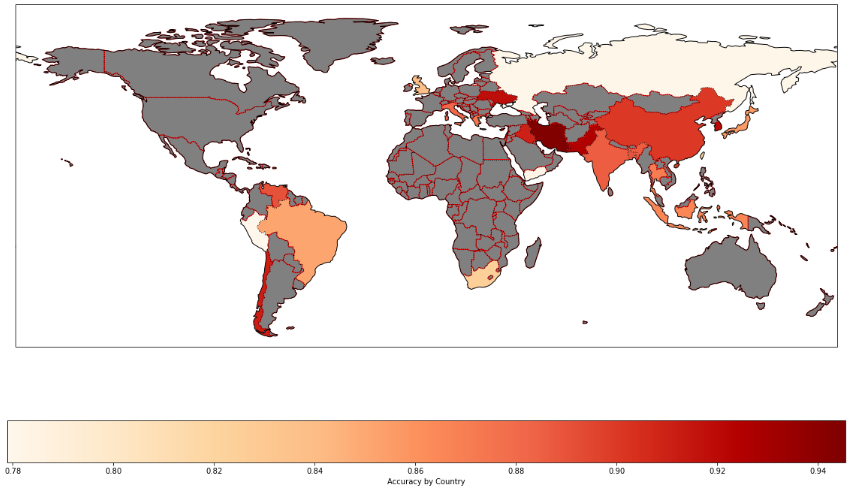
\includegraphics[width=0.75\linewidth]{Figures/global_accuracy_by_country.png}
    \caption{Map of 24 countries included in validation testing.  Each country in the validation testing has a minimum of 100 images.}
    \label{fig:global_map_validation}
\end{figure}


\begin{table}
    \centering
    \begin{tabular}{|l|l|}
        \hline
        \textbf{Test Accuracy}  & \textbf{89.41\%} \\  \hline
        True Positives (predict riot) & 2,903 \\       \hline
        False Positives & 345 \\   \hline
        False Negatives (missed riot) & 342 \\  \hline
        True Negatives & 2,900 \\  \hline
        \hline
        Precision & 89.38\% \\        \hline
        Recall & 89.46\% \\        \hline
        F1 Score & 89.42\%  \\
        \hline
    \end{tabular}
    \caption{Results from validation testing.}
    \label{tab:validation_global_results}
\end{table}



\begin{table}
\centering
\begin{tabular}{|l|l|l|l|l|l|l|}
\hline
\textbf{Country} & \textbf{Count}& \textbf{Accuracy} & \textbf{TP} & \textbf{FP} & \textbf{TN} & \textbf{FN} \\ \hline
Lebanon        & 330  & 94.54\% & 159 & 12 & 153 & 6  \\ \hline
Iran           & 466  & 94.42\% & 225 & 18 & 215 & 8  \\ \hline
Pakistan       & 524  & 92.56\% & 247 & 24 & 238 & 15 \\ \hline
South Korea    & 1498 & 92.12\% & 700 & 69 & 680 & 49 \\ \hline
Ukraine        & 184  & 91.85\% & 84  & 7  & 85  & 8  \\ \hline
Chile          & 260  & 91.15\% & 120 & 13 & 117 & 10 \\ \hline
Iraq           & 100  & 91.00\% & 45  & 4  & 46  & 5  \\ \hline
China          & 310  & 90.00\% & 140 & 16 & 139 & 15 \\ \hline
Palestine      & 314  & 89.49\% & 141 & 17 & 140 & 16 \\ \hline
Venezuela      & 128  & 89.06\% & 58  & 8  & 56  & 6  \\ \hline
Bangladesh     & 218  & 88.99\% & 90  & 5  & 104 & 19 \\ \hline
India          & 228  & 88.60\% & 97  & 9  & 105 & 17 \\ \hline
Italy          & 144  & 88.19\% & 62  & 7  & 65  & 10 \\ \hline
Greece         & 126  & 87.30\% & 62  & 15 & 48  & 1  \\ \hline
Thailand       & 178  & 87.08\% & 75  & 9  & 80  & 14 \\ \hline
Indonesia      & 134  & 86.57\% & 62  & 13 & 54  & 5  \\ \hline
Japan          & 250  & 85.60\% & 105 & 16 & 109 & 20 \\ \hline
Brazil         & 222  & 85.14\% & 94  & 16 & 95  & 17 \\ \hline
United Kingdom & 112  & 83.93\% & 50  & 12 & 44  & 6  \\ \hline
South Africa   & 296  & 82.43\% & 114 & 18 & 130 & 34 \\ \hline
Taiwan         & 112  & 82.14\% & 45  & 9  & 47  & 11 \\ \hline
Yemen          & 120  & 78.33\% & 41  & 7  & 53  & 19 \\ \hline
Russia         & 132  & 78.03\% & 50  & 13 & 53  & 16 \\ \hline
Peru           & 104  & 77.88\% & 37  & 8  & 44  & 15 \\ \hline
\end{tabular}
    \caption{Results from country level accuracy after validation testing.  These results are listed from highest accuracy to lowest accuracy.  We have also included the number of True Positives (TP), False Positives (FP), True Negatives (TN), and False Negatives (FN) for each country. }
    \label{tab:validation_country_results}
\end{table}

Of note, we observe a strong correlation between our softmax classification scores and accuracy within each country around the world, suggesting that softmax scores can be used as a proxy for prediction confidence (see figure \ref{fig:softmax_v_accuracy}).  While softmax may bias towards higher degrees of confidence \citep{pearce2021understanding, subramanya2017confidence}, as a relative metric it may provide helpful guidance to policymakers seeking to use these types of methods.

\begin{figure}
    \centering
    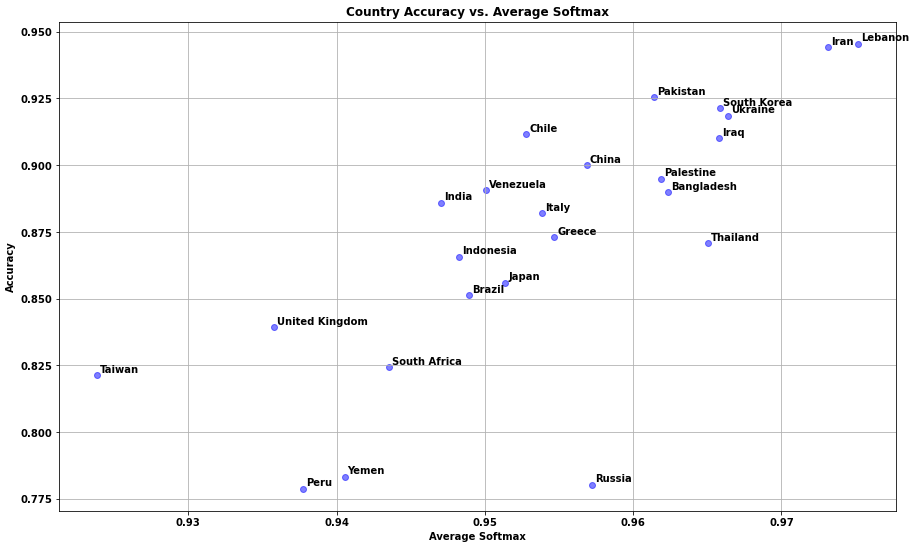
\includegraphics[width=0.75\linewidth]{softmax_v_accuracy.png}
    \caption{The average softmax for each country when compared to the average accuracy of prediction of each country.  Of note, the axis's do not begin at 0, but instead focus in on the domain and range of the values in the data.}
    \label{fig:softmax_v_accuracy}
\end{figure}


\subsection{Explainability of Results}

For our best performing model (model C in the table \ref{tab:fulldata_results_table}), we implemented Score-CAM on a subset of randomly selected, paired locations, ultimately consisting of 1,089 riot locations, and 1,089 null locations.  The Score-CAM results were then visually reviewed in an attempt to discern patterns in what the trained ResNet used in classification.  Interpreting the results of Score-CAM is inherently qualitative, making this a rich area for future work; we discuss this limitation further in section \ref{sec:explainability}.  
\par
Despite the limitations of Score-CAM, the visual interpretation indicated a few clear patterns.  An example of the first of these is displayed in figure \ref{fig:score_cam_stadium}, in which we can observe a large sports stadium in the image in the southeast region.  This large stadium is the location which Score-CAM identifies as the portion of the image which leads towards the classification (indicated through brighter values in the displayed heatmap).  In this case, the sports stadium lead the ResNet to classify the scene as a location that is unlikely to experience a riot.  We can see another example in figure \ref{fig:score_cam_stadium2}, in which again, the ResNet identifies the sports stadium as the reason to classify the scene as a non-riot.  We do not offer any explanation for why the sports stadiums are indicative of a non-riot scene, but these stadiums provide an example of the specific features which ResNet is learning to make classification decisions.  
\begin{figure}
    \centering
    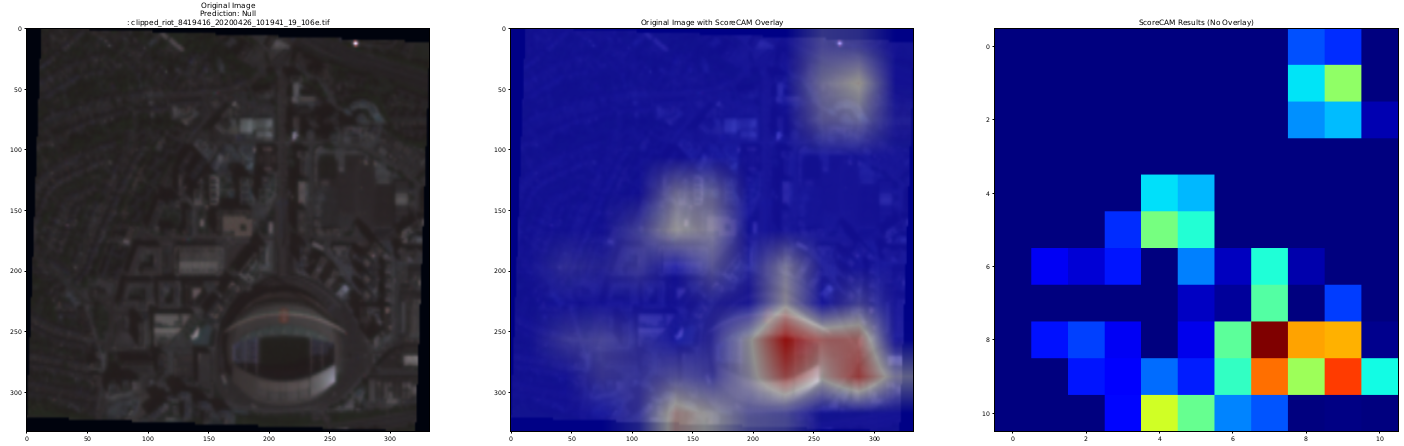
\includegraphics[width=1\linewidth]{scorecam_stadium.png}
    \caption{Example clipped image on the left.  The clipped image, a one kilometer box around a riot location.  The Score-CAM overlayed on top of the image is shown in the middle.  The Score-CAM visual is displayed on the right. Imagery \textcopyright Planet Labs PBC 2023. All rights reserved.}
    \label{fig:score_cam_stadium}
\end{figure}

\begin{figure}
    \centering
    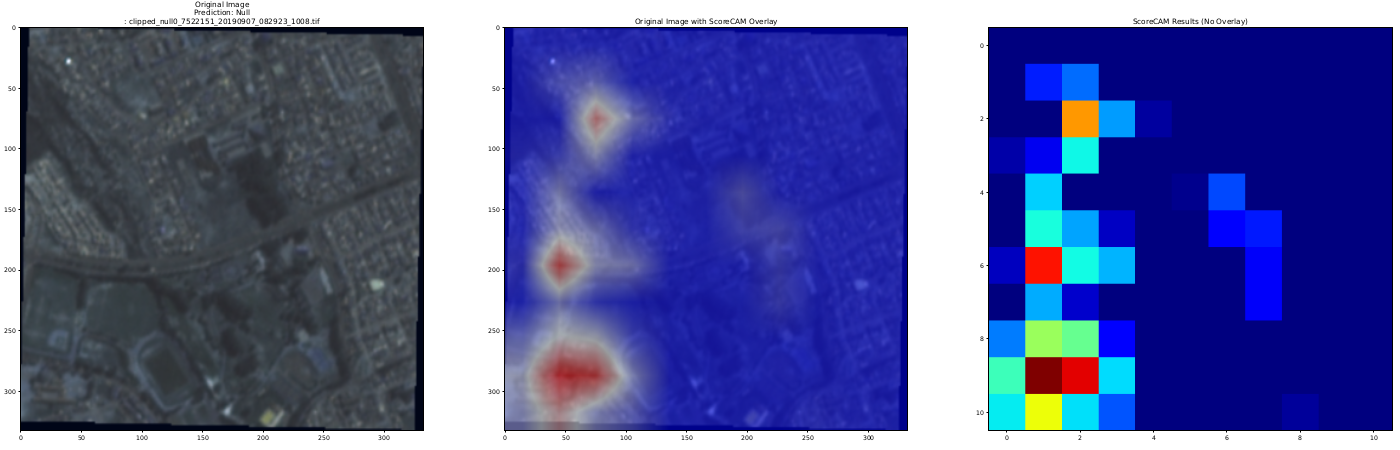
\includegraphics[width=1\linewidth]{stadium_scorecam2.png}
    \caption{Example clipped image on the left.  The clipped image, a one kilometer box around a non riot location.  The Score-CAM overlayed on top of the image is shown in the middle.  The Score-CAM visual is displayed on the right. Imagery \textcopyright Planet Labs PBC 2023. All rights reserved. }
    \label{fig:score_cam_stadium2}
\end{figure}

Another example highlighted in the Score-CAM analysis is shown in figure \ref{fig:fort_lalbagh}.  We can see a densely populated area, with a large open park or green space in the center of the image.  The trained network correctly predicted this image was from a riot or protest.  When we reference the ACLED data, this image is from a protest in the Lalbagh neighborhood of Dhaka, Bangladesh.  Lalbah is a fort built during the Mughal period in 1678, which was used subsequently by the British and Bangladesh governments as a location of governance and influence \citep{shakur2010culture}. Today, it is a location containing monument's and statues symbolizing rulers and regimes of the past, that is known as a common location for protests in the city of Dhaka \citep{begum2018changing}. While the deep learning model was not aware of these historic contexts, the unusual land use and associated image features were sufficient to classify this as a likely location of riots.

\begin{figure}
    \centering
    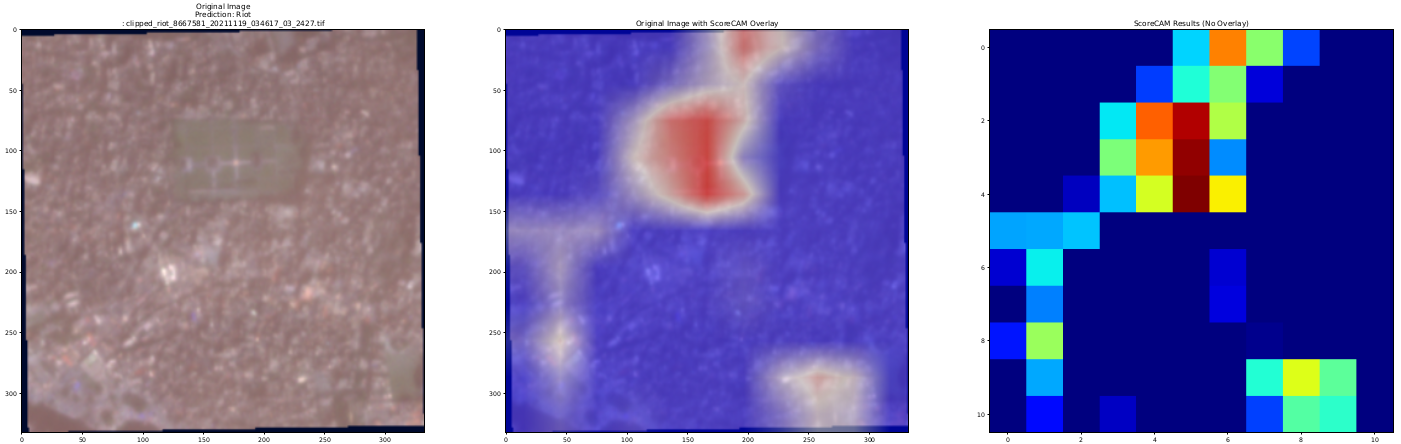
\includegraphics[width=1\linewidth]{fort_lalbagh_scorecam.png}
    \caption{The image on the left is a centered on Lalbagh Fort in Dhaka Bangladesh, taken on 19 November 2021, lesss than 48 hours before a protest at that location.  The Score-Cam visual is displayed on the right. Imagery \textcopyright Planet Labs PBC 2023. All rights reserved. }
    \label{fig:fort_lalbagh}
\end{figure}

\section{Discussion and Conclusions}
The results presented in table \ref{tab:fulldata_results_table} provide evidence that satellite information alone can provide useful information for the purposes of predicting where, within an urban environment, protests and riots are most likely to occur.  While this finding is likely to be of interest to those operating in data-sparse environments, it is well supported by past social science literature highlighting the interconnected nature of urban form and social processes \citep{fox2016urban,begum2018changing}.  By engaging in a global-scope study, here we are able to exploit this correlation by learning what these patterns are, and then leveraging them in estimation.  This finding held true across multiple model and data permutations (see tables \ref{tab:fulldata_results_table}, \ref{tab:validation_global_results} and \ref{tab:validation_country_results}), indicating that - even in some of the most challenging situations (i.e., relatively small training and validation sets), model accuracy can approach or exceed 90\%.

Furthermore, this technique performs well across the globe.  As highlighted in figure \ref{fig:global_map_validation}, there do not seem to be any regions that under perform.  Many countries with a relative low accuracy score (i.e., Russia) are in close proximity to a country with a higher accuracy score (i.e., China).  This pattern holds across the globe in South America, Asia, the Middle East, and Europe. 

Of note, in our softmax analysis seeking to correlate scores to accuracy, a single outlier, Russia, is observed in figure \ref{fig:softmax_v_accuracy} and table \ref{tab:validation_country_results}.  Russia has a lower comparative accuracy to other countries with similar softmax results.  This might be indicative of Russia's control of news sources \citep{gehlbach2010reflections}, or inherit bias in ACLED's collection of data which relies on news sources and non-governmental observation organizations that might not be focused on Russia.





\subsection{Conclusions}
In this work we constructed a data set consisting of 204,941 satellite images of riots and protests across the world.  After subseting the images into two classes of riots and non-riots, we trained a ResNet18 to identify which images were from locations associated with a riot.  When fine-tuned, our model achieved an accuracy of over 97\%, suggesting that satellite imagery has information of relevance and value to estimating the location of riot events.  This was true across a wide range of different tests and permutations of the data. We further provide some initial exploration into the explainability of this model, leveraging ScoreCAM to identify features the model is using in the classification task.


\section{Supplemental Information}\label{sec:appendix}



\subsection{Deduplication Tests}\label{sec:limited_data_set}

In this section, we present a test that controls for both class imbalance and geographic bias in our data. Our methodology leverages a large set of training data, specifically relying on an arbitrary 10:1 ratio of 10 null cases (no conflict event) to 1 positive case (a location where a conflict occurred).  Furthermore, some geographic locations are in the database multiple times - i.e., there may have been multiple protests at the same geographic location, even if they are at different dates (see table \ref{tab:occurrence}).  This results in both class imbalance (10 null cases for every 1 positive case), and geographic biases in where events are drawn from.  The class imbalance will potentially inflate accuracy scores, given a 10 to 1 ratio of null clips to riot clips - i.e., an untrained model could simply predict null for all images, and achieve an accuracy of 90.9\%.  Additionally, with repeated locations, the model will see the riot clip locations multiple times (i.e., even when each satellite scene has unique spatial information as it is drawn from a different date, the 1-km box centered on the latitude and longitude of the neighborhood will be the same).  This might allow our network to learn the specifics of a location, and over-fit to particular locations, instead of learning what features in urban areas predict riots and protests.  Therefore we constructed a limited data set to control for these issues.

To test if these attributes of our data resulted in bias, a new dataset was constructed which limited the data to a single riot image (1,089 1-km boxes) and a single non-riot image (1,089 1-km boxes) per location.  This means that our model was only able to analyze a riot location a single time during training, regardless of how frequently riots might happen at that location.  This should be a much harder training task for the model, with far less data available (2,178 images in total; these 2,178 images represent roughly 1\% of the data available for training in the full data set of 204,941 images).  Under these constraints, the maximum classification accuracy we observed was 67.37\% (see table \ref{tab:singleloc_results_table}).  Of note, the recall scores for our full data set and limited data set were very similar (75.18\% and 77.0\% respectively), despite the different size and scope of the training data.  

These results suggest that - even under extremely challenging, small-N circumstances - deep learning models can still identify meaningful features that are correlated with protest and riot events from satellite imagery.  


% Given the imbalance in our full data set, we also created a smaller data set without an imbalance.  In this smaller data set, there is only a single riot clip and single null clip per location.  We have also removed any repeated locations, creating a balanced data set with 1,089 riot clips and 1,089 null clips.  This is a more challenging scenario for training, because the model will only see each location a single time, and there is significantly less data available for training.  Even given the challenging scenario outlined, with this smaller data set the model performed well, achieving 65.57\% accuracy.  More detailed results can be seen in figure \ref{fig:singleloc_chart} and in table \ref{tab:singleloc_results_table}.  

% \begin{figure}
%     \centering
%     \includegraphics[width=0.5\linewidth]{singlelocation_finetuned.png}
%     \caption{Testing loss (in orange) and training loss (in blue) for the fine tuned model.  These results represent training the same fine tuned hyper parameter set, but only allowing a single riot clip and a single null riot clip per location.}
%     \label{fig:singleloc_chart}
% \end{figure}

\begin{table}
    \centering
    \begin{tabular}{|l|l|}
        \hline
        \textbf{Test Accuracy}  & \textbf{65.37\%} \\
        \hline
        True Positives (predict riot) & 154 \\
        \hline
        False Positives & 105 \\
        \hline
        False Negatives (missed riot) & 46 \\
        \hline
        True Negatives & 131 \\
        \hline
        \hline
        Precision & 59.46\% \\
        \hline
        Recall & 77.0\% \\
        \hline
        F1 Score & 67.1\%  \\
        \hline
    \end{tabular}
    \caption{Results from ResNet18 using only a single riot clip and single null riot clip per location.}
    \label{tab:singleloc_results_table}
\end{table}

\subsection{All Results} \label{large_table_of_results}
While we focus on our best performing models throughout this piece, there were a number of additional permutations and tests we performed while identifying the best modeling strategies, which we present here.  We began grid search across select hyperparameters, using a small test set of 100 random samples from our full data set.  Initially we were concerned with narrowing down the selection of the best performing learning rates, freezing layers of the ResNet, and dropping out connections between our fully connected layers.  The results of a sample of these are shown in table \ref{tab:initial_gridsearch_100A} and table \ref{tab:initial_gridsearch_100B}.  

\begin{table}
\centering
\begin{tabular}{|l|l|l|l|l|l|l|}
\hline
Metric & A1 & A2 & B1 & B2 & C1 & C2 \\ \hline
\hline
Test Accuracy (\%) & 91.59 & 91.12 & 90.65 & 93.93 & 93.46 & 86.45 \\\hline
\hline
True Positives & 0 & 0 & 0 & 0 & 0 & 0 \\ \hline
False Positives & 0 & 0 & 4 & 0 & 0 & 0 \\ \hline
False Negatives & 18 & 19 & 16 & 13 & 14 & 29 \\ \hline
True Negatives & 196 & 195 & 194 & 201 & 200 & 185 \\ \hline
\hline
Precision (\%) & 0.00 & 0.00 & 0.00 & 0.00 & 0.00 & 0.00 \\ \hline
Recall (\%) & 0.00 & 0.00 & 0.00 & 0.00 & 0.00 & 0.00 \\ \hline
F1 Score (\%) & 0.00 & 0.00 & 0.00 & 0.00 & 0.00 & 0.00 \\ \hline
\hline
Learning Rate & 1e-06 & 1e-06 & 1e-06 & 1e-06 & 1e-06 & 1e-06 \\ \hline
Freeze Layers & 0 & 0 & 5 & 5 & 10 & 10 \\ \hline
Drop Out Pair & (0, 0) & (0.1, 0.05) & (0, 0) & (0.1, 0.05) & (0, 0) & (0.1, 0.05) \\ \hline
L2 Weight Decay & 0 & 0 & 0 & 0 & 0 & 0 \\ \hline
\hline
\end{tabular}
\caption{All of the models in this table were tested with 100 random locations (100 riot clips and 1,000 null clips). In this table, all models used a learning rate of 1e-06. Models froze either none of the ResNet layers (A1, A2), the first 5 layers (B1, B2), or the first 10 layers (C1, C2). Between the first two and the second two layers, none of the connections were dropped (A1, B1, C1), or 10\% and 5\% were dropped (A2, B2, C2). }


\label{tab:initial_gridsearch_100A}
\end{table}



\begin{table}
\centering
\begin{tabular}{|l|l|l|l|l|l|l|}

\hline
Metric & D1 & D2 & E1 & E2 & F1 & F2 \\ \hline
\hline
Test Accuracy (\%) & 88.78 & 86.92 & 91.12 & 91.59 & 88.32 & 88.78 \\ \hline
True Positives & 5 & 1 & 7 & 5 & 0 & 0 \\ \hline
False Positives & 7 & 13 & 4 & 6 & 0 & 0 \\ \hline
False Negatives & 17 & 15 & 15 & 12 & 25 & 24 \\ \hline
True Negatives & 185 & 185 & 188 & 191 & 189 & 190 \\ \hline
\hline
Precision (\%) & 41.67 & 7.14 & 63.64 & 45.45 & 0.00 & 0.00 \\ \hline
Recall (\%) & 22.73 & 6.25 & 31.82 & 29.41 & 0.00 & 0.00 \\ \hline
F1 Score (\%) & 29.41 & 6.67 & 42.42 & 35.71 & 0.00 & 0.00 \\ \hline
\hline
Learning Rate & 1e-05 & 1e-05 & 1e-05 & 1e-05 & 1e-05 & 1e-05 \\ \hline
Freeze Layers & 0 & 0 & 5 & 5 & 10 & 10 \\ \hline
Drop Out Pair & (0, 0) & (0.1, 0.05) & (0, 0) & (0.1, 0.05) & (0, 0) & (0.1, 0.05) \\ \hline
L2 Weight Decay & 0 & 0 & 0 & 0 & 0 & 0 \\ \hline
\hline
\end{tabular}
\caption{All of the models in this table were tested with 100 random locations (100 riot clips and 1,000 null clips). In this table, all models used a learning rate of 1e-05. Models froze either none of the ResNet layers (D1, D2), the first 5 layers (E1, E2), or the first 10 layers (F1, F2). Between the first two and the second two layers, none of the connections were dropped (D1, E1, F1), or 10\% and 5\% were dropped (D2, E2, F2).}
\label{tab:initial_gridsearch_100B}
\end{table}

After the initial grid search, we increased the size of data set to 1,000 locations (1,000 riot clips, and 10,000 null clips).  We also adjusted the hyperparameter grid search space.  Our best performing model referred to as Model C in table \ref{tab:hyper_param_search}, is Config 10 in table \ref{tab:initial_gridsearch_1000B}.  Config 10 has the highest F1 Score across these grid search results, reflecting the best balance between Precision and Recall.  Due to this strong performance, these parameters were used to train the full dataset.


\begin{table}
\centering
\begin{tabular}{|l|l|l|l|l|l|l|}
\hline
Metric & Config 1 & Config 2 & Config 3 & Config 4 & Config 5 & Config 6 \\ \hline
\hline
Test Accuracy (\%) & 91.80 & 91.80 & 91.27 & 90.69 & 92.52 & 91.85 \\ \hline
True Positives & 62 & 39 & 43 & 77 & 25 & 78 \\ \hline
False Positives & 54 & 11 & 41 & 65 & 7 & 62 \\ \hline
False Negatives & 116 & 159 & 140 & 128 & 148 & 107 \\ \hline
True Negatives & 1,841 & 1,864 & 1,849 & 1,803 & 1,893 & 1,826 \\ \hline
\hline
Precision & 0.5345 & 0.7800 & 0.5119 & 0.5423 & 0.7812 & 0.5571 \\ \hline
Recall & 0.3483 & 0.1970 & 0.2350 & 0.3756 & 0.1445 & 0.4216 \\ \hline
F1 Score & 0.4218 & 0.3145 & 0.3221 & 0.4438 & 0.2439 & 0.4800 \\ \hline
\hline
Learning Rate & \multicolumn{6}{c|}{1e-05} \\ \hline
L2 Weight Decay & \multicolumn{3}{c|}{0.1} & \multicolumn{3}{c|}{0.01} \\ \hline
Freeze Layer & 0 & 0 & 0 & 5 & 5 & 5 \\ \hline
Dropout Pair & (0, 0) & (0.1, 0.05) & (0.5, 0.1) & (0, 0) & (0.1, 0.05) & (0.5, 0.1) \\ \hline

\end{tabular}
\caption{Model performance metrics for configurations 1 to 6 with learning rate of 1e-05, with variations in L2 weight decay, freeze layer, and dropout pair settings.}
\label{tab:initial_gridsearch_1000A}
\end{table}


\begin{table}
\centering
\begin{tabular}{|l|l|l|l|l|l|l|}
\hline
Metric & Config 7 & Config 8 & Config 9 & Config 10 & Config 11 & Config 12 \\ \hline
\hline
Test Accuracy (\%) & 91.51 & 89.77 & 92.91 & 92.33 & 90.16 & 92.76 \\ \hline
True Positives & 85 & 86 & 54 & 86 & 92 & 80 \\ \hline
False Positives & 64 & 106 & 34 & 32 & 101 & 49 \\ \hline
False Negatives & 112 & 106 & 113 & 127 & 103 & 101 \\ \hline
True Negatives & 1,812 & 1,775 & 1,872 & 1,828 & 1,777 & 1,843 \\ \hline
\hline
Precision & 0.5705 & 0.4479 & 0.6136 & 0.7288 & 0.4767 & 0.6202 \\ \hline
Recall & 0.4315 & 0.4479 & 0.3234 & 0.4038 & 0.4718 & 0.4420 \\ \hline
F1 Score & 0.4913 & 0.4479 & 0.4235 & 0.5196 & 0.4742 & 0.5161 \\ \hline
\hline
Learning Rate & \multicolumn{6}{c|}{1e-05} \\ \hline
L2 Weight Decay & \multicolumn{3}{c|}{0.01} & \multicolumn{3}{c|}{0.001} \\ \hline
Freeze Layer & 0 & 0 & 0 & 5 & 5 & 5 \\ \hline
Dropout Pair & (0, 0) & (0.1, 0.05) & (0.5, 0.1) & (0, 0) & (0.1, 0.05) & (0.5, 0.1) \\ \hline

\end{tabular}
\caption{Model performance metrics for configurations 7 to 12 with learning rate of 1e-05, transitioning from L2 weight decay settings of 0.01 to 0.001, including variations in freeze layer and dropout pair settings.}
\label{tab:initial_gridsearch_1000B}
\end{table}






\begin{figure}
    \centering
    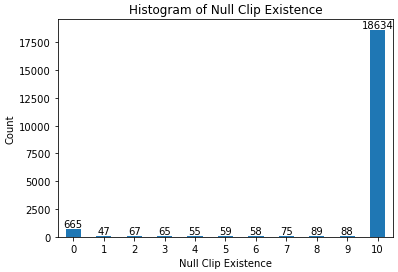
\includegraphics[width=0.5\linewidth]{null_clip_histogram.png}
    \caption{Distribution of null clips from the full 19,902 images downloaded.  Instances where less than 10 clips were taken are primarily due to the amount of urban area available in the satellite image.  There were three additional locations that were eventually able to provide 10 null clips, but not included before the dataset was finalized with 18,631 locations at training time.}
    \label{fig:null_hist}
\end{figure}





